\documentclass[12pt]{report}

% Información
\title{Proyecto 2: Base de Datos Musical}
\author{Angel de Jesus Gervacio Martinez}

% Paquetes
\usepackage[spanish]{babel}
\usepackage[margin=1in]{geometry}
\usepackage{url}
\usepackage{fancyhdr}
\usepackage{float}
\usepackage{graphicx}
\usepackage[dvipsnames]{xcolor}
\usepackage{titlesec}
\usepackage{tikz}
\usepackage{tabularx}
\usepackage{listings}
\usepackage{tcolorbox}
\usepackage{caption}
\usepackage{lscape}
\usepackage{titlesec}
\usepackage{etoolbox}

% Estilo de pagina
\pagestyle{fancy}
\fancyhead[LO, L]{\textbf{Proyecto 2: Base de Datos Musical}}
\fancyhead[RO, R]{\textbf{Modelado y Programación}}
\fancyfoot[LO, L]{\textbf{Facultad De Ciencias, 2027-1}}
\fancyfoot[CO, C]{\textbf{\thepage}}
\fancyfoot[RO, R]{\textbf{UNAM}}
\renewcommand{\headrulewidth}{1pt}
\renewcommand{\footrulewidth}{1pt}

\titleformat{\chapter}[block]
  {\normalfont\Large\bfseries}
  {\thechapter}
  {1em}
  {}

\titlespacing*{\chapter}
  {0pt}
  {0pt}
  {0.5em}

\makeatletter
\patchcmd{\chapter}{\if@openright\cleardoublepage\else\clearpage\fi}{}{}{}
\makeatother

% Inicio del documento
\begin{document}

% Portada
\begin{titlepage}
  \begin{center}
    % Inicio
    \textbf{\large\uppercase{Universidad Nacional Autónoma de México}}\\[0.4cm]
    \textbf{\large\uppercase{Facultad De Ciencias, 2027-1}}\\[0.4cm]
    \textbf{\large\uppercase{Modelado y Programación}}\\[0.4cm]

   
    \begin{figure}[htb]
      \begin{center}
        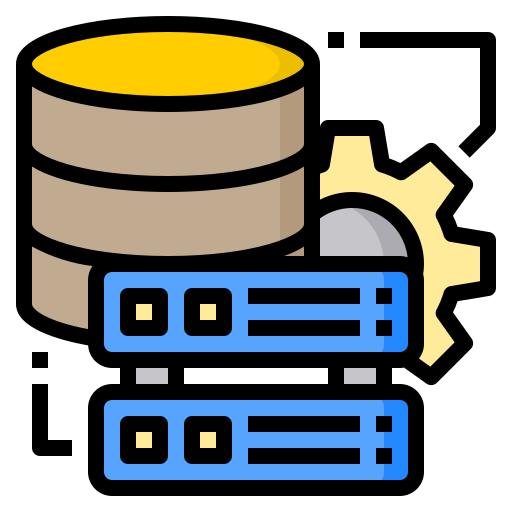
\includegraphics[scale=1]{icono_datos.png}\\
      \end{center}
    \end{figure}
    
    % Titulo
    \rule{\linewidth}{1pt}\\[0.4cm]
    \color{CadetBlue}
    \large\uppercase{\textbf{Proyecto 2:}}\\[0.2cm]
    \color{Black}
    \textbf{\Large\uppercase{Base de Datos Musical}}\\[0.2cm]
    \rule{\linewidth}{1pt}\\[0.8cm]
  \end{center}
\end{titlepage}

\chapter{Resumen}
En este proyecto se desarrollo una \textbf{base de datos musical} la cual se divide en varios componentes como la \textbf{base de datos}, \textbf{minero}, \textbf{interfaz gráfica} y un \textbf{compilador}.\\

Mediante la \textit{interfaz gráfica} el usuario puede minar los metadatos de archivos MP3, puede editar, eliminar u obtener la información de la base de datos sin tener que escribir SQL directamente, además, puede reproducir los archivos minados.\\

Para la realización de este proyecto se utilizaron herramientas como \textbf{Meson}, \textbf{Qt}, \textbf{Doxygen} y la biblioteca \textbf{SQLite} y fue implementado en el lenguaje \textit{C++}.\\

De esta forma se logro tener una forma en la que el usuario puede acceder a los archivos MP3 que se encuentran en sus sistema de forma organizada y de facil acceso.\\

\chapter{Introducción}
El proyecto se realizo para la materia de \textit{Modelado y Programación}, haciendo aplicacion de temas como análisis y diseño, interfaces gráficas, patrones de diseño y principalmente una introducción al manejo de bases de datos.\\

Como principal proposito del proyecto se busca que los estudiantes, hagan uso de patrones de diseño en sus proyectos, empezar a reconocerlos y darse cuenta en que partes vitales de sus proyectos pueden aplicarlos para facilitar el desarrollo de estos, por otro lado, también se busca que aprendan sobre el desarrollo de interfaces gráficas y su interacción con el usuario.\\

Las dificultades que se pueden presentar a lo largo de desarrollo se presentan principalmente en la forma de implementar y ajustar a las necesidades del proyecto los patrones de diseño, además de las repercusiones que dicha implementación puede tener en un desarrollo más avanzado del proyecto, llegando a tener que recurrir a algun otro patron de diseño o tener que hacer un cambio drastico por algun elemento no contemplado en el análisis y desarrollo del proyecto.\\

En el caso de la interfaz gráfica, resulta necesario tener que aprender las formas en las que se puede tanto diseñar e implementar. Además, debe de ser intuitiva y facil de usar para cualquier usuario.\\

Por otro lado durante la implementación, puede ser necesario utilizar alguna biblioteca que ayude y facilite el desarrollo del proyecto, sin embargo, hacer uso de las bibliotecas no siempre es tan sencillo, pues puede ser necesario tener que cumplir algunos requisitos como tener que instalar otras bibliotecas o tener que modificar nuestro proyecto, afectando tanto al análisis como al diseño que ya teniamos planeado o incluso la implementanción que ya se tenia hecha.\\

Al finalizar el proyecto, con la experiencia que los estudiantes tuvieron, se espera que a futuro les sea más sencillo su desarrollo o incluso que decidan usar otros recursos para comparar cual puede ser más util y en que casos es mejor hacer uso de ellos.\\

En este punto, podran notar diferencias notables con proyectos implementandos en materias cursadas con anterioridad, podran tener en cuenta lo aprendido para mejorarlos o podrian darles una nueva utilidad usandolos como base de proyectos que combinados con las nuevas herramientas que han aprendido seran de gran utilidad tanto para si mismos como otras personas.\\

\chapter{Análisis y diseño}
\section{Análisis}
Con la información inicial dada de el proyecto, podemos dividirlo en cuatro partes principales:\\

Necesitamos un \textbf{Minero} el cual dado un directorio debe poder identificar los archivos MP3, analizar los que cuenten con etiquetas \textit{Id3v2.4}, dicho \textit{Minero} tiene que funcionar recursivamente, es decir, poder leer los subdirectorios, además, debe de inferir la información como los albumes de las canciones que tendran como ruta los directorios donde se encuentren los MP3.\\

Otra de las partes principales es la \textbf{Interfaz Gráfica}, esta sera la vista del usuario, mediante la cual podra ver la base de datos, y podra editar la información como el titulo, año o el interprete de una canción, entre otros.\\

Los cambios realizados por el usuario solo se guardan en la base de datos no en los metadatos de los archivos MP3.\\

Tenemos también la \textbf{Base de Datos}, que tiene un esquema definido y la cual con ayuda de el \textit{Minero} poblara la \textit{Base de Datos}.\\

Debido a el esquema, podemos tener \textit{rolas} las cuales cuentan con un número de identificación, asi como el número de identificación de su interprete y de su album, también cuentan con una ruta, titulo, año, número de pista y genero.\\

Tambien tenemos \textit{interpretes} los cuales tienen un número de identificación, su tipo de interprete y su nombre. Tenemos tres tipo de interprete, los cuales son \textit{persona}, \textit{grupo} o \textit{desconocido}.\\

Las \textit{personas} tienen un número de identificación, nombre artistico, nombre real, fecha de nacimiento y fecha de fallecimiento.\\

Para los \textit{grupos}, estos cuentan con un número de identificación, nombre, fecha de formación y fecha de separación, tienen miembros los cuales son \textit{personas}, entonces podemos agregar \textit{personas} que no tengan relación con ninguna \textit{rola} de la base de datos, y podemos asociarlas a los grupos.\\

Por ultimo, tenemos el \textbf{Compilador}, este mediante un pequeño lenguaje permitira realizar busquedas por diversos campos, sin que el usuario tenga que escribir SQL directamente.\\

\section{Diseño}
Con la información recabada en el análisis, resulta más sencillo realizar el diseño de el proyecto y podemos definir los atributos y comportamientos de quienes participan en la \textit{Base de Datos Musical}.\\

\subsection{Base de Datos}
Para esta parte tenemos una clase \textbf{AdministraBD} la cual se encargara de abrir la \textit{Base de Datos} y permitir el acceso a esta.\\

Para hacer más sencillo el acceso a los datos consultados tendremos las clases: \textbf{Metadatos} (debido a la cantidad de atributos, hace uso de el patron de diseño \textit{Builder}), \textbf{Artista}, \textbf{Album}, \textbf{Persona} y \textbf{Banda}, de esta forma agrupamos todos los atributos.\\

Para poder agregar, editar y consultar datos, haremos uso de el patron de diseño \textit{Data Access Object}, al principio del desarrollo se tenia planeado utilizar una unica clase para la implementación, sin embargo, debido a la cantidad de datos que se manejan es más sencillo tener cinco clases las cuales son: \textbf{CancionesDAO}, \textbf{ArtistasDAO}, \textbf{AlbumsDAO}, \textbf{BandasDAO} y \textbf{PersonasDAO}.\\

\begin{figure}[H]
  \begin{center}
    \makebox[\textwidth][c]{
      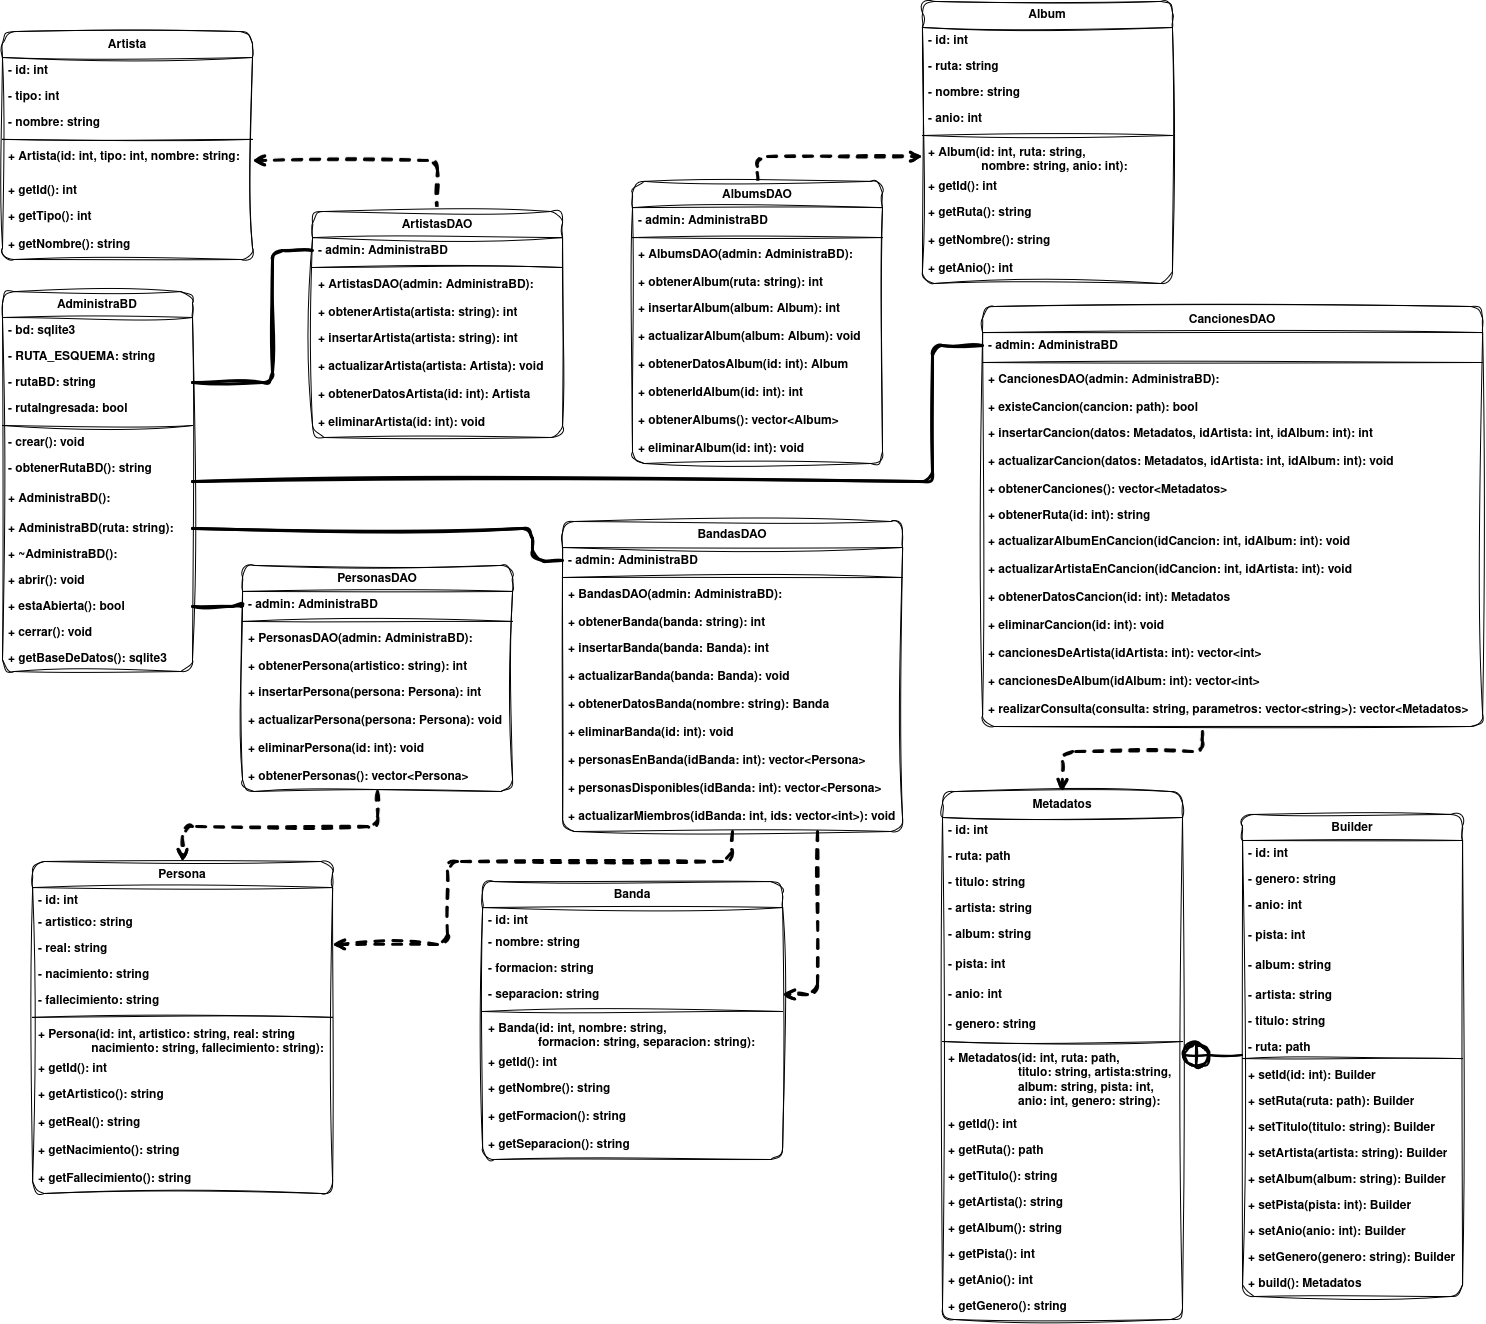
\includegraphics[width=1.2\textwidth]{BaseDatos.png}
    }
  \end{center}
\end{figure}

\subsection{Minero}
Para el \textit{Minero} tenemos una sola clase, la cual recorre el directorio dado y sus subdirectorios, ademas de poder leer las etiquetas \textit{Id3v2.4} de los archivos MP3, y con dicha información se podra poblar la \textit{Base de Datos} haciendo uso de las clases DAO anteriormente mencionadas.\\

\begin{figure}[H]
  \begin{center}
    \makebox[\textwidth][c]{
      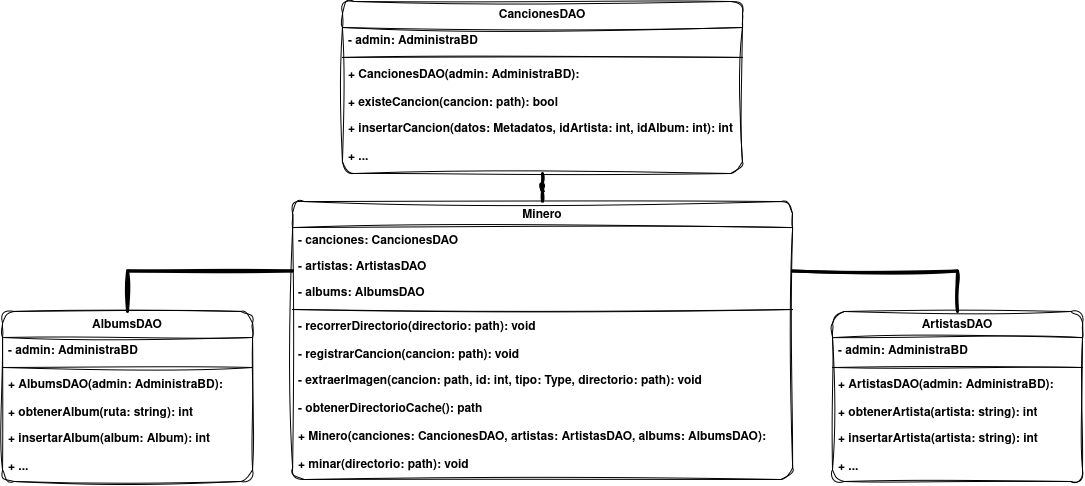
\includegraphics[width=1.2\textwidth]{Minero.png}
    }
  \end{center}
\end{figure}

\subsection{Compilador}
Para el \textit{Compilador}, podemos dividirlo en varias clases las cuales son: \textit{Token}, \textit{Lexer}, \textit{Vertice}, \textit{Parser}, \textit{ValidadorSemantico}, \textit{Generador} y una clase \textit{Compilador} que hara uso de las clases anteriores.\\

La clase \textit{Lexer} recibira la cadena de texto con la busqueda y al recorrerla obtendra una lista de \textit{Token}, la cual es recibida por la clase \textit{Parser}, esta se encargara de generar el árbol de sintaxis abstracta de la busqueda, y el \textit{ValidadorSemantico} se encargara de revisar que la semantica de la busqueda sea valida, es decir, que tenga logica y sea posible realizar la consulta, una vez que se compruebe su validez, el \textit{Generador} recibira el árbol y con este generara la consulta SQL que se tiene que realizar, además regresara una lista con los parametros de la consulta, finalmente todo el proceso sera organizado desde la clase \textit{Compilador}.\\

Como se menciono en el diseño se hara uso de un pequeño lenguaje para realizar busquedas, este se define de la siguiente forma:\\

\begin{verbatim}
CONSULTA = "@@" , EXPRESION

EXPRESION = TERMINO , { "||" , TERMINO }

TERMINO = FACTOR , { "&&" , CONDICION }

CONDICION = CONDICION_TEXTO | CONDICION_NUMERICA

CONDICION_TEXTO = CAMPO_TEXTO , OPERADOR_TEXTO , TEXTO

CONDICION_NUMERICA = CAMPO_NUMERICO , OPERADOR_NUMERICO , NUMERO

CAMPO_TEXTO = "ARTISTA" | "ALBUM" | "RUTA" | "TITULO" | "GENERO"

CAMPO_NUMERICO = "PISTA" | "AÑO"

OPERADOR_TEXTO = "=" | "!=" | "~="

OPERADOR_NUMERICO = "=" | "!=" | ">=" | ">" | "<=" | "<"

TEXTO = '"' , { CARACTER } , '"'

CARACTER = LETRA | DIGITO | " " | SIMBOLO 

LETRA = "A"..."Z" | "a"..."z" | "Á" | "É" | "Í" | "Ó" | "Ú" | "Ü" | "Ñ"
      | "á" | "é" | "í" | "ó" | "ú" | "ü" | "ñ"

NUMERO = "0" | DIGITO_NO_CERO, { NUMERO }

DIGITO_NO_CERO = "1" ... "9"

SIMBOLO = "_" | "-" | "." | "/" | "\" | ":" | ";" | "," | "!" | "?" | "@"
        | "#" | "$" | "%" | "&" | "*" | "+" | "~" | "^" | "'" | "(" | ")"

\end{verbatim}

Podemos tener entonces busquedas como:\\

\begin{verbatim}        
@@ARTISTA="Queen"&&AÑO=1980
\end{verbatim}

Esta busqueda regresara todas las canciones de el grupo \textit{Queen} y que su año sea igual a \textit{1980}.\\

\begin{verbatim}        
@@TITULO~="Love"
\end{verbatim}        

Esta busqueda regresara todas las canciones que contengan en el titulo \textit{Love}.\\

\begin{verbatim}        
@@ALBUM!="Magic"||AÑO>=2000
\end{verbatim}

Esta busqueda regresara todas las canciones que su album no sea \textit{Magic} ó que su año sea mayor o igual a \textit{2000}.\\

\begin{figure}[H]
  \begin{center}
    \makebox[\textwidth][c]{
      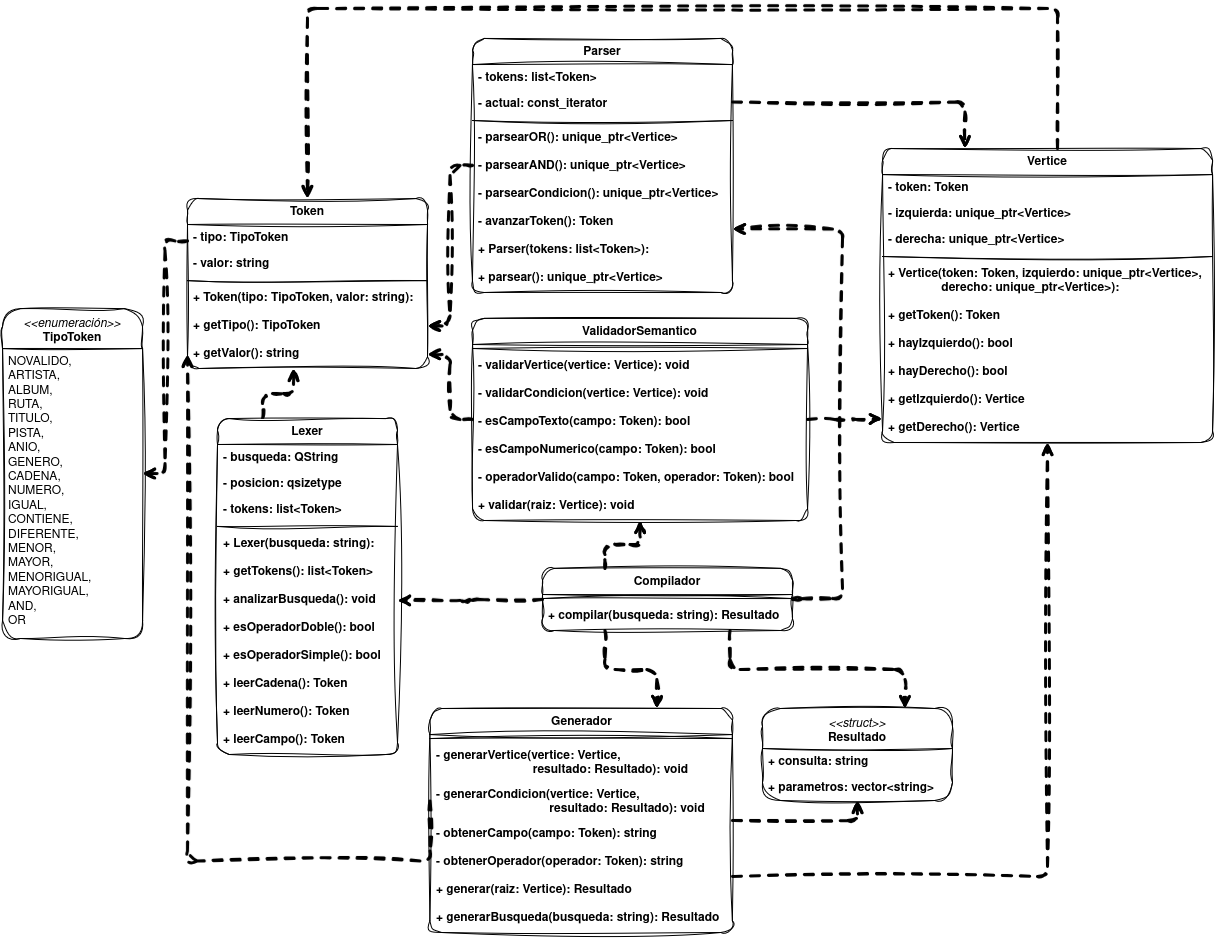
\includegraphics[width=1.2\textwidth]{Compilador.png}
    }
  \end{center}
\end{figure}

\subsection{Interfaz Gráfica}
Para la \textit{Interfaz Gráfica} se hara uso de el patron de diseño \textit{Modelo-Vista-Controlador}, por lo cual necesitaremos una clase \textit{Controlador}, la vista podra hacer uso de los metodos de esta clase y el \textit{Controlador} hara uso de las clases de el modelo, las cuales seran las clase que hacen uso de el patron de diseño \textit{Data Access Object} para interactuar con la \textit{Base de Datos}.\\

Por otro lado tendremos una clase \textit{CancionesModelo} que sera de utilidad para poder representar la \textit{Base de Datos} dentro de la interfaz, y también tendremos una clase \textit{Reproductor} que servira para reproducir las canciones mediante su ruta en el sistema, se podra cambiar de canción, pausar la reproducción y cambiar el volumen.\\

Las clases \textit{Controlador} y \textit{Reproductor} haran uso de señales para comunicarse con la interfaz, cuando se complete con exito algun cambio de volumen, duracion, actualizar la información de canciones, artistas, albums, entre otros, si ocurre algun error durante la ejecución también se usara una señal que tendra el mensaje del error ocurrido.\\

\begin{figure}[H]
  \begin{center}
    \makebox[\textwidth][c]{
      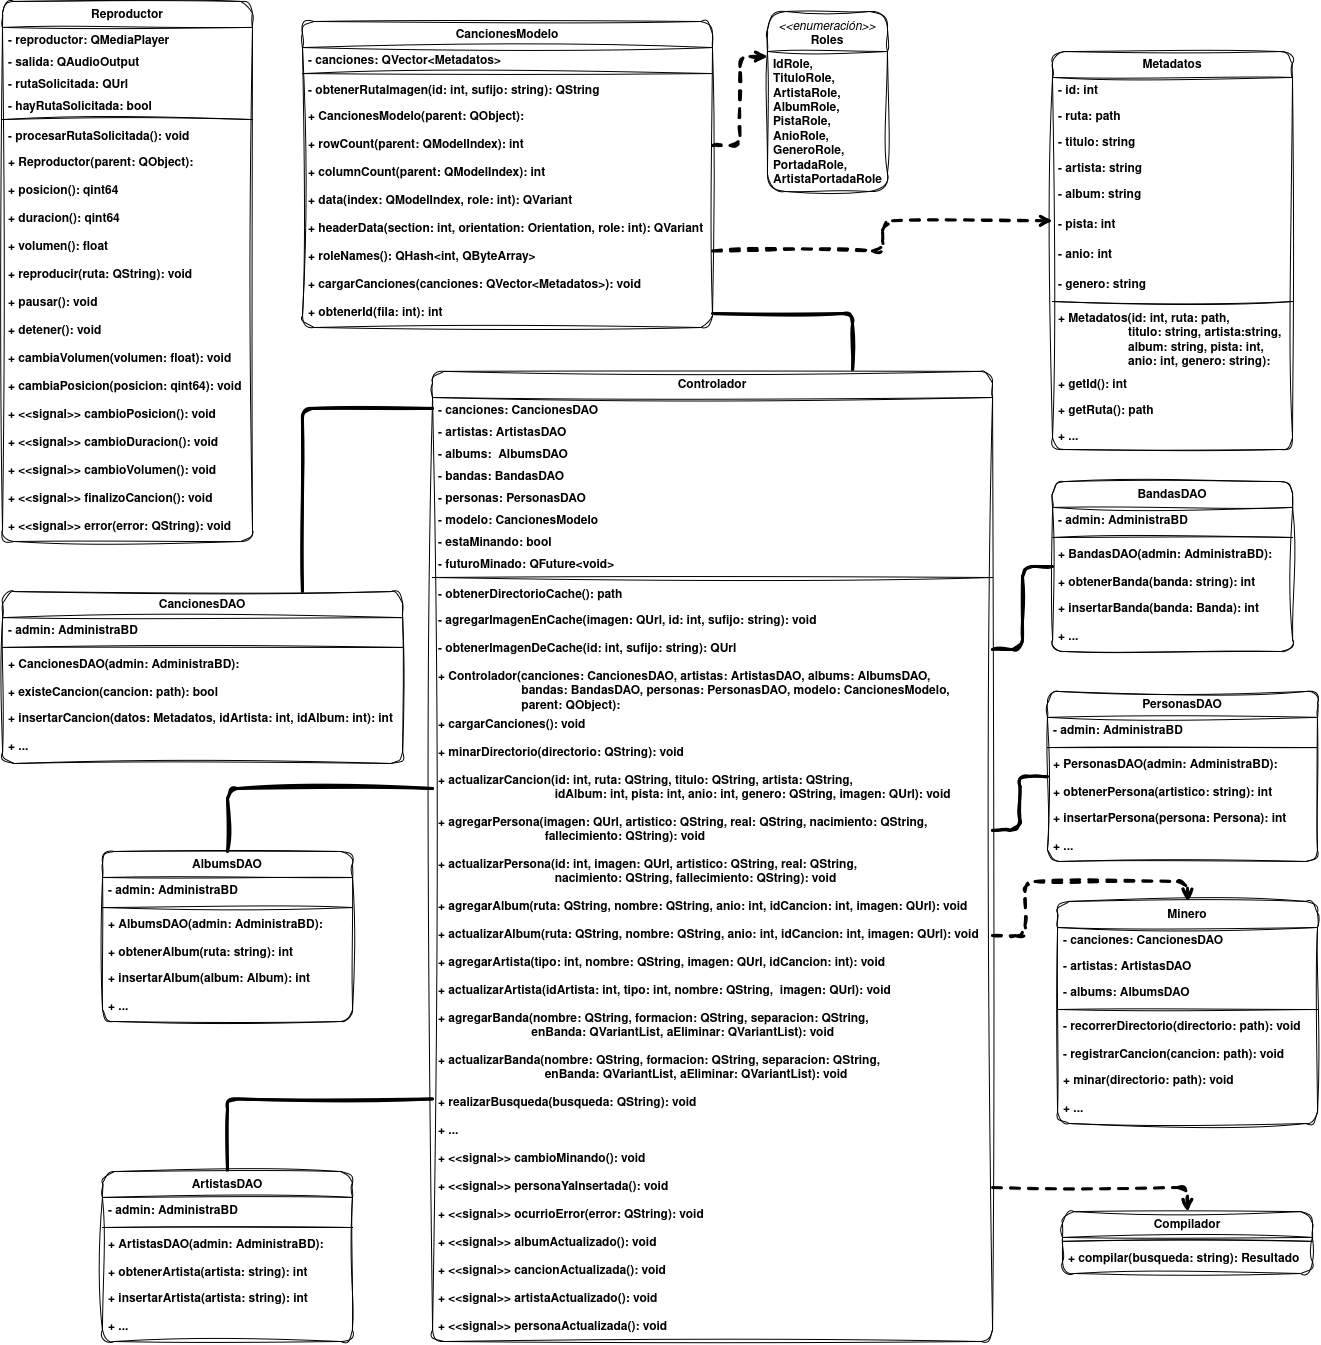
\includegraphics[width=1.1\textwidth]{Interfaz.png}
    }
  \end{center}
\end{figure}

\chapter{Implementación}
Con las clases ya definidas en el diseño podemos pasar a la implementación.\\

Haremos uso de el sistema de construcción \textit{Meson}, este nos permitira compilar el proyecto, generar los ejecutables y ejecutar pruebas unitar usando también \textit{GoogleTest}.\\

Comenzamos implementando las clases relacionadas con la \textit{Base de Datos}, pues son las que usaremos a menudo durante el desarrollo, para ello hacemos uso de la biblioteca \textit{SQLite} que permitira realizar las consultas en la \textit{Base de Datos} de manera sencilla.\\

Una vez implementadas las clases, procedemos con el \textit{Minero}, para esta clase haremos uso de la biblioteca \textit{TagLib} (que hace uso de la biblioteca \textit{utfcpp}), con esta obtendremos los metadatos de los archivos MP3 y con las clases de la \textit{Base de Datos} agregamos la información a la base de datos.\\

A continuación procedemos con la implementación de la \textit{Interfaz Gráfica} la cual se desarrollara con \textit{Qt} y su lenguaje de marcado declarativo \textit{QML}, una vez definidos todos los archivos \textit{QML} y agregar las imagenes para botones y placeholders, podemos proceder a darle funcionalidad a la \textit{Interfaz Gráfica}, por lo cual implementamos el \textit{Controlador}, \textit{CancionesModelo} y \textit{Reproductor}.\\

Una vez que la \textit{Interfaz Gráfica} pueda funcionar sin errores hara falta poder realizar busquedas, por lo cual procedemos a implementar el \textit{Compilador} y sus clases, de esta forma podemos obtener la consulta necesaria para realizar la busqueda en la \textit{Base de Datos}.\\

Finalmente, podemos realizar cambios en el codigo para mejorarlo o simplificarlo, podemos inclusive deshacernos de metodos que no terminamos usando en el productor final.\\

\section{Ejecución}
Las versiones indicadas corresponden a las utilizadas durante el desarrollo y no representan versiones mínimas.\\

El proyecto utiliza \textit{Meson (1.4.1)}, \textit{Ninja (1.12.1)}, \textit{g++ (14.2.1)} y \textit{Qt (6.8.2)}. Además, requiere GoogleTest, SQLite3, TagLib y utfcpp, las cuales pueden instalarse automáticamente mediante los \textit{wraps} incluidos en el proyecto, aunque esto incrementa el tiempo de compilación. También se requiere Doxygen (1.10.0) para generar la documentación.\\

Para compilar el proyecto y ejecutar las pruebas unitarias, primero se clona el repositorio y posteriormente se ejecutan los siguientes comandos:\\

\begin{verbatim}
git clone https://github.com/AngelGervacio/Proyecto2-BDMusical.git
meson setup build
meson compile -C build
sudo meson install -C build
meson test -C build
\end{verbatim}

El proyecto genera dos ejecutables: \textit{Minero} para minar los directorios y llenar la base de datos desde la terminl, se ejecuta de la forma \textbf{./build/src/Minero -d /ruta/}, donde \textit{-d} indica el directorio que se analizará y \textit{-b} permite especificar la ubicación de la base de datos, y \textit{BDMusical} que abre la interfaz gráfica del proyecto, se ejecuta como \textbf{./build/src/gui/BDMusical}.\\

Finalmente, la documentación se genera con \textbf{doxygen Doxyfile} y puede consultarse en \textbf{docs/html/index.html}.\\

Para consultar los requisitos de forma más detallada, se recomienda consultar el archivo \textit{README.md} incluido en el repositorio del proyecto.\\

\chapter{Conclusiones}
En un inicio, pense que se me dificultaria realizar este proyecto, principalmente por el manejo de la base de datos, sin embargo, con la experiencia que tuve de el proyecto anterior, me resulto más sencillo poder investigar como realizar la implementación de algunas partes de el codigo en \textit{C++}.\\

Una vez que entendi como hacer uso de las bibliotecas mediante su documentación, se me hizo más sencillo continuar el proyecto, de manera que la mayor parte de el proyecto fue enfocada en la implementación de la interfaz gráfica con Qt y el resultado que obtuve fue de mi agrado.\\

Debido a la gran cantidad de metodos que implemente y el tiempo no me fue posible realizar por completo las pruebas unitarias, aunque algunas podrian ser similares a las de otros métodos.\\

\chapter{Bibliografia}

\url{https://www.doxygen.nl/manual/index.html}

\url{https://www.freecodecamp.org/news/what-are-bnf-and-ebnf/}

\url{https://www.geeksforgeeks.org/compiler-design/phases-of-a-compiler/}

\url{https://google.github.io/googletest/}

\url{https://mesonbuild.com/}

\url{https://doc.qt.io/qt-6.8/}

\url{https://www.sqlite.org/docs.html}

\url{https://taglib.org/}
\end{document}
